% Copyright 2020-2022 Robert Bosch GmbH

% Licensed under the Apache License, Version 2.0 (the "License");
% you may not use this file except in compliance with the License.
% You may obtain a copy of the License at

% http://www.apache.org/licenses/LICENSE-2.0

% Unless required by applicable law or agreed to in writing, software
% distributed under the License is distributed on an "AS IS" BASIS,
% WITHOUT WARRANTIES OR CONDITIONS OF ANY KIND, either express or implied.
% See the License for the specific language governing permissions and
% limitations under the License.

\hypertarget{description-get-robotframework-xml-result}{%
\section{Get \rfwcore\ XML result}
\label{description-get-robotframework-xml-result}}

\begin{boxhint}{Hint}
In case you have already had the \rfwcore\ *.xml result file(s), you can skip this section 
and move to \hyperref[description-tool-features]{Tool features} section to get what this 
tool can do with your \emph{*.xml} file(s).

However, you can also refer this section to understand the definitions of \rfwcore
\rcode{Metadata}information and their reflections when importing to TestResultWebApp's 
database.
\end{boxhint}

In order to get the \rfwcore\ \emph{*.xml} result file(s), we need to execute the Robot testcase
first, the below settings is recommended for Robot testcase. 
So that the generated \emph{*.xml} result file will contains all required information when 
displaying on TestResultWebApp.

\hypertarget{description-robotframework-testcase-settings}{%
\subsection{\rfwcore\ Testcase Settings}
\label{description-robotframework-testcase-settings}}

\begin{boxhint}{Hint}
The below document is common \rfwcore\ Testcase Settings before execution.
So that, the generated \emph{*.xml} result file will contain all required information for 
importing to TestResultWebApp's database.\\
\\
However, we suppose to use \rfw\ with 
\href{https://github.com/test-fullautomation/robotframework-testsuitesmanagement}
{RobotFramework\_Testsuites} library for executing Robot testcase(s).

It will help to define the below\rcode{Metadata}information implicitly within the 
\rcode{Suite Setup} bases on your environment and configuration in *.json file:
\begin{itemize}
  \item \rcode{project}
  \item \rcode{version\_sw}
  \item \rcode{version\_hw}
  \item \rcode{version\_test}
  \item \rcode{machine}
  \item \rcode{tester}
  \item \rcode{testtool}
\end{itemize}

So that, you do not need to define these\rcode{Metadata}in your Robot test case.
\end{boxhint}

For the whole test execution:

\begin{itemize}

\item Project/Variant

\begin{robotcode}
Metadata    project     ${Project_name}
\end{robotcode}

\item Versions

\begin{robotcode}
Metadata    version_hw     ${Software_version}
Metadata    version_hw     ${Hardware_version}
Metadata    version_test   ${Test_version}
\end{robotcode}
\end{itemize}

For the Suite/File information:
\begin{itemize}

\item Description/Documentation

\begin{robotcode}
Documentation   ${Suite_description}
\end{robotcode}

\item Author

\begin{robotcode}
Metadata   author   ${Author_name}
\end{robotcode}

\item Component
  
\begin{robotcode}
Metadata   component   ${Component_name}
\end{robotcode}

\item Test Tool - Test framework and Python version, e.g \textbf{Robot Framework
  3.2rc2 (Python 3.9.0 on win32)}

\begin{robotcode}
Metadata   testtool   ${Test_tool}
\end{robotcode}

\item Test Machine

\begin{robotcode}
Metadata   machine   %{COMPUTERNAME}
\end{robotcode}

\item Tester

\begin{robotcode}
Metadata   tester   %{USER}
\end{robotcode}

\end{itemize}

For test case information:

\begin{itemize}

\item Issue ID

\begin{robotcode}
[Tags]   ISSUE-${ISSUE_ID}
\end{robotcode}

\item Testcase ID

\begin{robotcode}
[Tags]   TCID-${TC_ID}
\end{robotcode}

\item Requirement ID

\begin{robotcode}
[Tags]   FID-${REQ_ID}
\end{robotcode}
\end{itemize}

\subsection{Sample \rfwcore\ Testcase}

Sample \rfwcore\ testcase with the neccessary information for importing to 
TestResultWebApp's database:

\begin{robotcode}[caption=Sample \rfwcore\ testcase,
                  linebackgroundcolor=\hlcode{3,4,5,6,12,13,14}]
*** Settings ***
# Test execution level
Metadata   project        ROBFW              # Project/Variant
Metadata   version_sw     SW_VERSION_0.1     # Software version
Metadata   version_hw     HW_VERSION_0.1     # Hardware version
Metadata   version_test   TEST_VERSION_0.1   # Test version

# File/Suite level
Documentation             This is description for robot test file
Metadata    author        Tran Duy Ngoan (RBVH/ECM1)
Metadata    component     Import_Tools
Metadata    testtool      Robot Framework 3.2rc2 (Python 3.9.0 on win32)
Metadata    machine       %{COMPUTERNAME}
Metadata    tester        %{USER}

*** Test Cases ***
Testcase 01
   [Tags]   ISSUE-001   TCID-1001   FID-112   FID-111
   Log       This is Testcase 01

Testcase 02
   [Tags]   ISSUE-RTC-003   TCID-1002   FID-113
   Log       This is Testcase 01
\end{robotcode}

\begin{boxhint} {Hint}
Above highlighted\rcode{Metadata}definitions are not required when using \rfw.

\href{https://github.com/test-fullautomation/robotframework-testsuitesmanagement}
{RobotFramework\_Testsuites} library will handle these definitions within \rcode{Suite Setup}.
\end{boxhint}

\subsection{Execute \rfwcore\ Testcase(s) to get result file}
Now, execute your Robot testcase(s) with your IDE or 
\href{https://robotframework.org/robotframework/latest/RobotFrameworkUserGuide.html#starting-test-execution}
{using command line} to get the Robot result file
\begin{robotlog}
robot your_testcases.robot
\end{robotlog}
Or with python module
\begin{robotlog}
python -m robot your_testcases.robot
\end{robotlog}

The default name of Robot result file is \emph{output.xml}. Its filename can be changed by 
specifying other filename with argurment \rlog{--output (-o)} when executing Robot 
testcase(s)
\begin{robotlog}
robot your_testcases.robot --output path/to/robot_result.xml
\end{robotlog}


\newpage
\hypertarget{description-tool-features}{%
\section{Tool features}\label{description-tool-features}}
After getting the \rfwcore\ \emph{*.xml} result file(s), you can use the \pkg\ tool to
import them into TestResultWebApp's database.

Its usage and enhance features are described as below.

\subsection{Usage}
Use below command to get tools's usage:
\begin{robotlog}
RobotLog2DB -h
\end{robotlog}

The tool's usage should be showed as below:
\begin{robotlog}
usage: RobotLog2DB (RobotXMLResult to TestResultWebApp importer) [-h] [-v] 
                   [--recursive] [--dryrun] [--append] [--UUID UUID] 
                   [--variant VARIANT] [--versions VERSIONS] [--config CONFIG]
                   resultxmlfile server user password database

RobotLog2DB imports XML result files (default: output.xml) generated by the Robot Framework 
                     into a WebApp database.

positional arguments:
resultxmlfile        absolute or relative path to the result file or directory of result
                     files to be imported.
server               server which hosts the database (IP or URL).
user                 user for database login.
password             password for database login.
database             database schema for database login.

optional arguments:
-h, --help           show this help message and exit
-v, --version        version of the RobotLog2DB importer.
--recursive          if set, then the path is searched recursively for output files to be 
                     imported.
--dryrun             if set, then verify all input arguments (includes DB connection) and 
                     show what would be done.
--append             is used in combination with --UUID <UUID>.If set, allow to append new 
                     result(s) to existing execution result UUID in --UUID argument.
--UUID UUID          UUID used to identify the import and version ID on webapp. 
                     If not provided RobotLog2DB will generate an UUID for the whole import.
--variant VARIANT    variant name to be set for this import.
--versions VERSIONS  metadata: Versions (Software;Hardware;Test) to be set for this import 
                     (semicolon separated).
--config CONFIG      configuration json file for component mapping information.
\end{robotlog}

As above instruction, \pkg\ tool requires 5 positional arguments which contains all required
information for inporting.\\
The below command is simple usage with all required arguments to import robot results into 
TestResultWebApp's database:
\begin{robotlog}
RobotLog2DB <output.xml> <localhost> <db\_user> <db\_pw> <db\_name>
\end{robotlog}

Besides the executable file \pkg\, you can also run tool as a Python module
\begin{robotlog}
python -m RobotLog2DB <output.xml> <localhost> <db\_user> <db\_pw> <db\_name>
\end{robotlog}

Beside the required arguments, there are optional arguments which provides some enhance
features as the following sections.

\subsection{Verify provided arguments}

Sometimes, we just want to validate the \emph{*.xml} and database
connection without changing anything in the database, the optional
argument \rlog{--dryrun} can be used in this case.

When executing in dryrun mode, \pkg\ will:

\begin{itemize}
\tightlist
\item
  Verify the provided \rfwcore\ \emph{*.xml} result file is valid or not.
\item
  Verify the database connection with provided credential.
\item
  Verify other information which given in optional arguments.
\item
  Just print all test cases will be imported without touching database.
\end{itemize}

This feature will helps you to ensure that there is no error when
executing \pkg\ tool (normal mode) to create new record(s) and
update TestResultWebApp's database.

\subsection{Searching *.xml result file(s)}

\pkg\ accepts the first arugment \rlog{resultxmlfile} can be a
single file or the folder that contains multiple result files.

When the folder is used, \pkg\ will only search for
\emph{*.xml} file under given directory and exclude any file within
subdirectories as default.

In case you have result file(s) under the subdirectory of given folder
and want these result files will also be imported, the optional arugment
\rlog{--recursive} should be used when executing \pkg\ command.

When \rlog{--recursive} argument is set, \pkg\ will walk
through the given directory and its subdirectories to discover and
collect all available \emph{*.xml} for importing.

For example: your result folder has a structure as below:

\begin{robotlog}
logFolder
   |_____ result_1.xml
   |_____ result_2.xml
   |_____ subFolder_1
   |         |________ result_sub_1.xml
   |         |________ subSubFolder
   |                       |______ result_sub_sub_1.xml
   |_____ subFolder_2
             |________ result_sub_2.xml
\end{robotlog}

\begin{itemize}
\tightlist
\item
  Without \rlog{--recursive}: only \textbf{result\_1.xml} and
  \textbf{result\_2.xml} are found for importing.
\item
  With \rlog{--recursive}: all \textbf{result\_1.xml},
  \textbf{result\_2.xml}, \textbf{result\_sub\_1.xml},
  \textbf{result\_sub\_2.xml} and \textbf{result\_sub\_sub\_1.xml} will
  be imported.
\end{itemize}

\subsection{Handle missing information}
\subsubsection{Default values}
TestResultWebApp requires \rcode{Project}, \rcode{version_sw} to manage the execution 
results and \rcode{component} to group test cases in the displayed charts.

In case above information is missing in 
\hyperref[description-robotframework-testcase-settings]{testcase settings} during the test 
case execution, that leads to the missing information in the \emph{output.xml} result file.
So, these missing information will be set to default value when importing with
\href{https://github.com/test-fullautomation/robotframework-robotlog2db}{\pkg} tool:

\begin{itemize}
\tightlist
\item \rlog{Project}: will be set to default value \pcode{ROBFW} if not defined.

\item \rlog{Software version}: will be set to execution time \pcode{\%Y\%m\%d\_\%H\%M\%S} 
                               as default value.

\item \rlog{Component}: will be set to default value \pcode{unknown} if not defined.
\end{itemize}

\subsubsection{Specify missing information with optional arguments}
But, you can also provide the missing information as command arguments when executing the
\href{https://github.com/test-fullautomation/robotframework-robotlog2db}{\pkg} tool with 
below optional arguments:

\begin{boxwarning}{Warning}
These below settings may overwrite the existing information of\rlog{project},
\rlog{version_sw}and\rlog{component}which have been defined in Robot testcase in 
\hyperref[description-robotframework-testcase-settings]{above settings}.
\\
So, \textbf{only} use these arguments in cases you want to define the missing information or 
overwrite them with your expected values for the importing result.
\end{boxwarning}

\begin{itemize}
\item \rlog{--variant VARIANT}

  To specify the \textbf{Project/Variant} information.

\item \rlog{--versions VERSIONS}

  To specify the \textbf{Software, Hardware} and \textbf{Test} versions information.

\item \rlog{--config CONFIG}

  To provide a configuration \emph{*.json} file as \pcode{CONFIG} argument.
  Currently, the configuration \emph{*.json} supports below settings:

  \begin{itemize}
  \item \rcode{"variant"} to specify the \textbf{Project/Variant} as \pcode{string} value.
  \item \rcode{"version_sw"} to specify the \textbf{Software version} information as \pcode{string} value.
  \item \rcode{"version_hw"} to specify the \textbf{Hardware under-test version} as \pcode{string} value.
  \item \rcode{"version_test"} to specify the \textbf{Test version} as \pcode{string} value.
  \begin{boxhint} {Notice}
    These above settings with \rlog{--config CONFIG} will have lower priority than the 
    commandline arguments \rlog{--variant VARIANT} and \rlog{--versions VERSIONS}
  \end{boxhint}
  \item \rcode{"testtool"} to specify the \textbf{Test toolchain} as \pcode{string} value.
  \item \rcode{"tester"} to specify the \textbf{Test user} as \pcode{string} value.
  \item \rcode{"components"} to specify the \textbf{Component} information which will be 
        displayed on \href{https://github.com/test-fullautomation/testresultwebapp}
        {TestResultWebApp}. Value can be:
        \begin{itemize}
          \item 
            \pcode{string}: to specify the same \emph{component} for all testcase
            within this execution.
\begin{robotcode}
{
  "components" : "atest",
  ...
}
\end{robotcode}
          \item
            \pcode{object}: to specify the mapping between \emph{component} info
            and \emph{classname} of testcase.
\begin{robotcode}
  {
    "components" : {
      "cli"       : "robot/cli",
      "core"      : "robot/core",
      "external"  : "robot/external",
      "keywords"  : "robot/keywords",
      "libdoc"    : "robot/libdoc",
      "connectivity" : [
          "selftest/serial",
          "selftest/ssh",
          "selftest/tcpip"
      ]
    },
    ...
  }
\end{robotcode}
        \end{itemize}
        The error will be occurred when the provided configuration
        \emph{*.json} schema is not correct.
  \end{itemize}
\end{itemize}

Sample configuration json file:

\begin{pythoncode}
{
   "components" : {
                  "cli"       : "robot/cli",
                  "core"      : "robot/core",
                  "external"  : "robot/external",
                  "keywords"  : "robot/keywords",
                  "libdoc"    : "robot/libdoc",
                  "connectivity" : [
                      "selftest/serial",
                      "selftest/ssh",
                      "selftest/tcpip"
                  ]
   },
   "version_sw" : "Atest",
   "variant"    : "ROBFW"
}
\end{pythoncode}

As above sample configuration, the component mapping can be explained as below:

\begin{itemize}
  \item Testcase(s) which path file contains \textbf{robot/cli} is belong to component \textbf{cli}
  \item Testcase(s) which path file contains \textbf{robot/core} is belong to component \textbf{core}
  \item Testcase(s) which path file contains \textbf{robot/external} is belong to component \textbf{external}
  \item Testcase(s) which path file contains \textbf{robot/keywords} is belong to component \textbf{keywords}
  \item Testcase(s) which path file contains \textbf{robot/libdoc} is belong to component \textbf{libdoc}
  \item And component \textbf{connectivity} contains all testcases which path file contains
        \textbf{selftest/serial}, \textbf{selftest/ssh} or \textbf{selftest/tcpip}.
\end{itemize}

\hypertarget{append-to-existing-execution-result}{%
\subsection{Append to existing execution result}\label{append-to-existing-execution-result}}

\pkg\ also allow you to append new test result(s) (missing from previous import, 
on other test setup, ...) into the existing execution result (identified by the 
\textbf{UUID}) in TestResultWebApp's database. 
The combination of optional arguments \rlog{--UUID <UUID>} and \rlog{--append} 
should be used in this case.

The \rlog{--append} makes \pkg\ run in append mode and the \rlog{--UUID <UUID>} 
will specify the existing UUID of execution result to be appended.

For example, the result with UUID \textbf{c7991c07-4de2-4d65-8568-00c5556c82aa} 
is already existing in TestResultWebApp's database and you want to append
result(s) in \textbf{output.xml} into that execution result.

The command will be used as below:

\begin{robotlog}
python -m RobotLog2DB output.xml localhost testuser testpw testdb --UUID c7991c07-4de2-4d65-8568-00c5556c82aa --append
\end{robotlog}

If the argument \rlog{--UUID <UUID>} is used without \rlog{--append}:

\begin{itemize}
  \item An error will be thrown and the import job is terminated immediately if 
        the provided \textbf{UUID} is already existing

\begin{robotlog}
FATAL ERROR: Execution result with UUID 'c7991c07-4de2-4d65-8568-00c5556c82aa' is already existing.
             Please use other UUID (or remove '--UUID' argument from your command) for new execution result.
             Or add '--append' argument in your command to append new result(s) to this existing UUID.
\end{robotlog}
  \item The importing execution result will have an identifier as the provided
        \textbf{UUID} if that \textbf{UUID} is not existing
\end{itemize}

If the argument \rlog{--append} is used and:
\begin{itemize}
  \item given UUID in \rlog{--UUID <UUID>} argument is existing: the new result(s) will be appended to that UUID
  \item given UUID in \rlog{--UUID <UUID>} argument is not existing: tool will be terminated immediately with below error
\begin{robotlog}
FATAL ERROR: Execution result with UUID 'c7991c07-4de2-4d65-8568-00c5556c82aa' is not existing for appending.
             Please use an existing UUID to append new result(s) to that UUID.
             Or remove '--append' argument in your command to create new execution result with given UUID.
\end{robotlog}
  \item \rlog{--UUID <UUID>} is not provided: tool will be terminated immediately with below error
\begin{robotlog}
FATAL ERROR: '--append' argument should be used in combination with '--UUID <UUID>` argument
\end{robotlog}
\end{itemize} 


\newpage
\hypertarget{description-display-on-webapp}{%
\section{Display on WebApp}\label{description-display-on-webapp}}

When the \emph{output.xml} file(s) is importing sucessfully to database, the result for that 
execution will be available on
\href{https://github.com/test-fullautomation/testresultwebapp}{TestResultWebApp}.

Above settings in robot testcase will be reflect on \textbf{Dashboard} (General view) and 
\textbf{Data table} (Detailed view) as below figures:

Execution result metadata:

\begin{figure}[h!]
  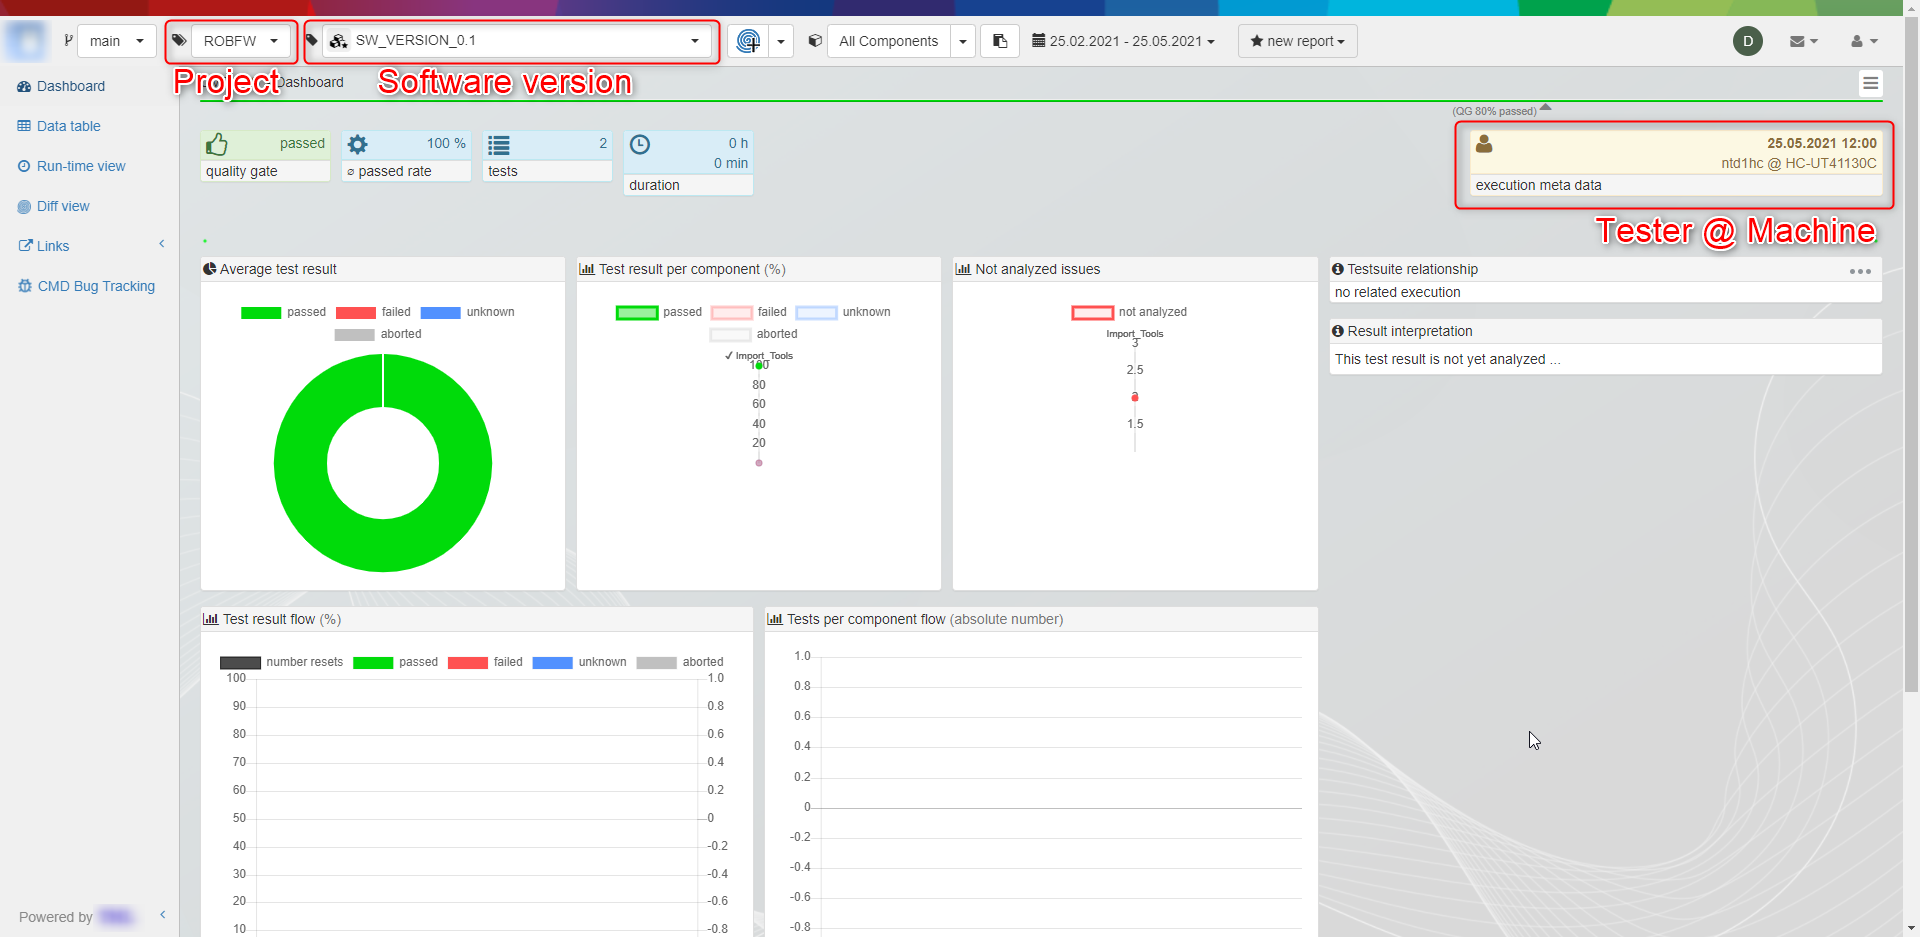
\includegraphics[width=1\linewidth]{./pictures/Dashboard.png}
  \caption{Dashboard view}
\end{figure}

Suite/File metadata and Testcase information:

\begin{figure}[h!]
  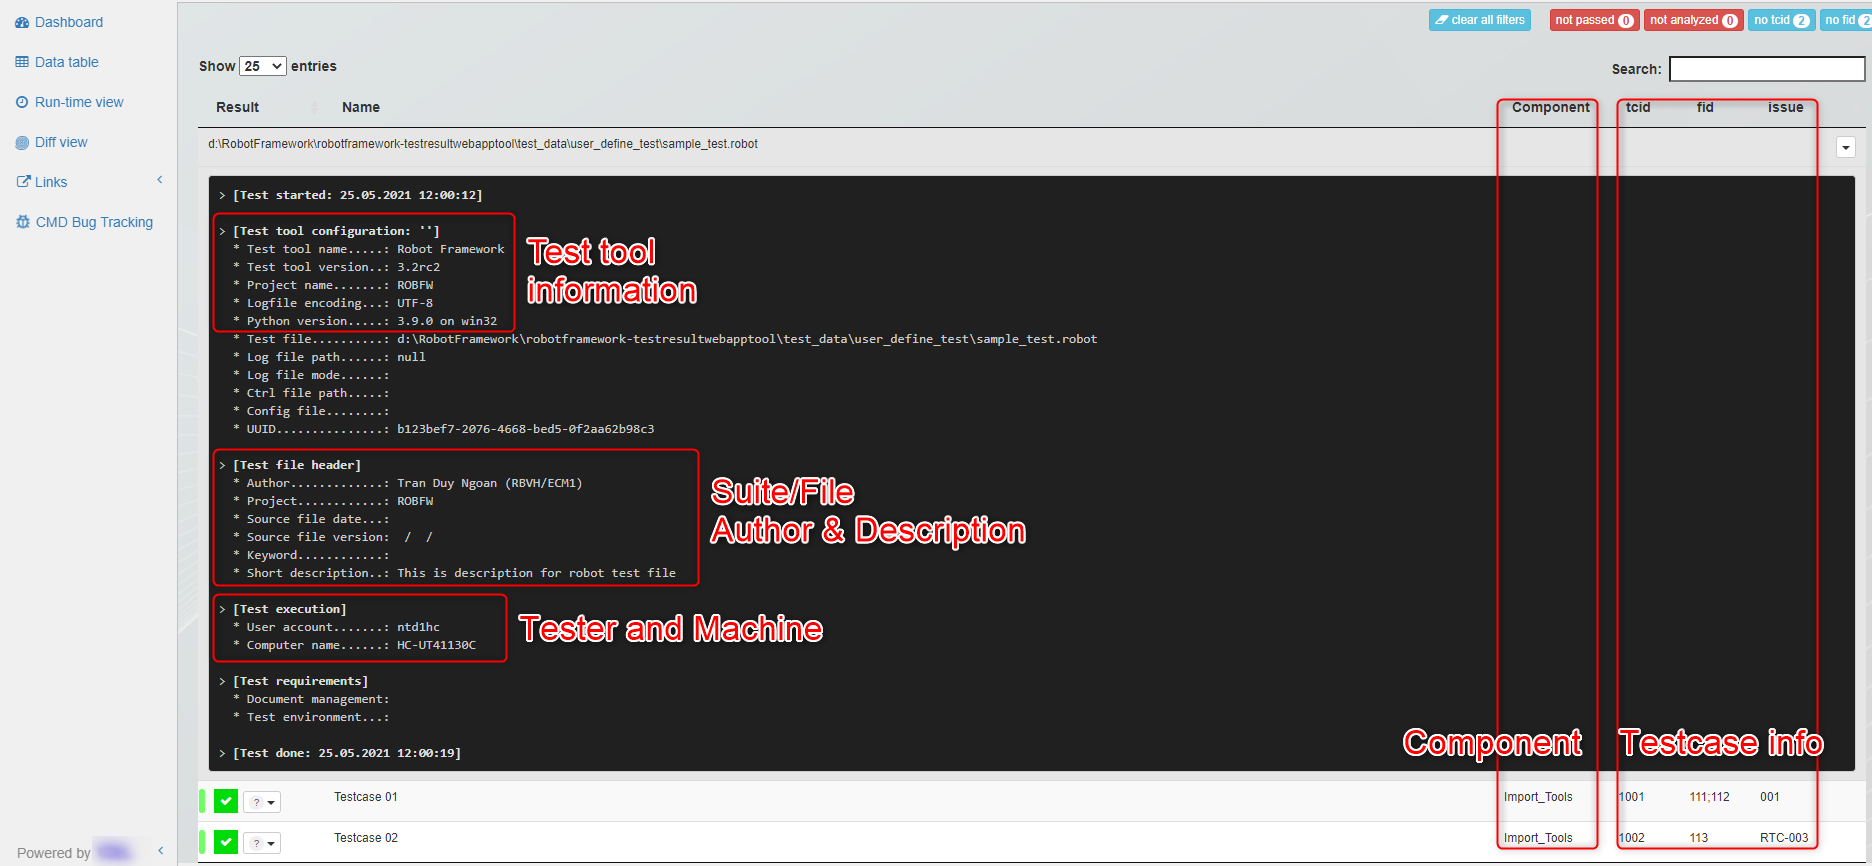
\includegraphics[width=1\linewidth]{./pictures/Datatable.png}
  \caption{Datatable view}
\end{figure}